\documentclass[crop,tikz]{standalone}

\tikzset{>=latex}

\def\wavelength{0.2}
\def\slitdistance{0.4}

\begin{document}
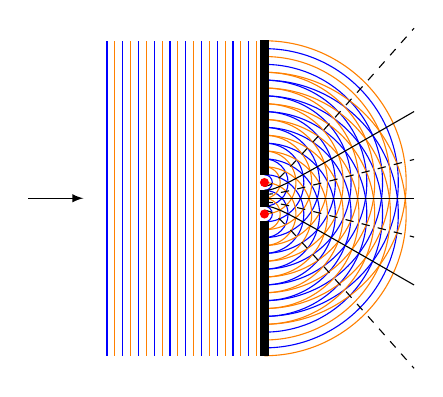
\begin{tikzpicture}
  % direction
  \draw[->] (-3,0) -- +(0.7,0);
  % coordinates of slits
  \coordinate (a) at (0,\slitdistance/2);
  \coordinate (b) at (0,-\slitdistance/2);
  % plain waves
  \foreach \X in {-2,-1.8,...,-0.2} {
    \draw[blue] (\X,-2) -- (\X,2);
    \draw[orange] (\X + \wavelength/2,-2) -- (\X + \wavelength/2,2);
  }
  % circular waves
  \foreach \r in {0.1,0.3,...,1.8} {
    \draw[blue] (a)+(-90:\r) arc (-90:90:\r);
    \draw[blue] (b)+(-90:\r) arc (-90:90:\r);
  }
  \foreach \r in {\wavelength,0.4,...,1.8} {
    \draw[orange] (a)+(-90:\r) arc (-90:90:\r);
    \draw[orange] (b)+(-90:\r) arc (-90:90:\r);
  }
  % lines of constructive interference
  \foreach \N in {-1,0,1} {
    \draw[domain=0:1.9,smooth,variable=\t] plot (\t,{(\N*\wavelength/2)*sqrt(1 + \t*\t/((\slitdistance/2)^2 - (\N*\wavelength/2)^2))});
  }
  % lines of destructive interference
  \foreach \N in {-2,-1,0,1} {
    \draw[domain=0:1.9,smooth,variable=\t,dashed] plot (\t,{((\N + 1/2)*\wavelength/2)*sqrt(1 + \t*\t/((\slitdistance/2)^2 - ((\N + 1/2)*\wavelength/2)^2))});
  }
  % aperture
  \draw[fill] (0.05,-2) rectangle (-0.05,-0.3);
  \draw[fill] (0.05,-0.1) rectangle (-0.05,0.1);
  \draw[fill] (0.05,2)  rectangle (-0.05,0.3);
  % red dots
  \draw[fill,red] (a) circle (0.05);
  \draw[fill,red] (b) circle (0.05);
\end{tikzpicture}
\end{document}
